\chapter{Results}
\label{chap:sidh}
As discussed in previous chapter, we implemented MSFC in ns3 to compare it to other traffic schedulers. We simulate part of wifi network an ISP may manage, since our scheduler aims to ordinary routers at the "last mile" of the Internet --- a few hops near the customer. We simulate several types of traffic common users generate and evaluate performance of a few traffic schedulers.

\begin{figure}
	\centering
	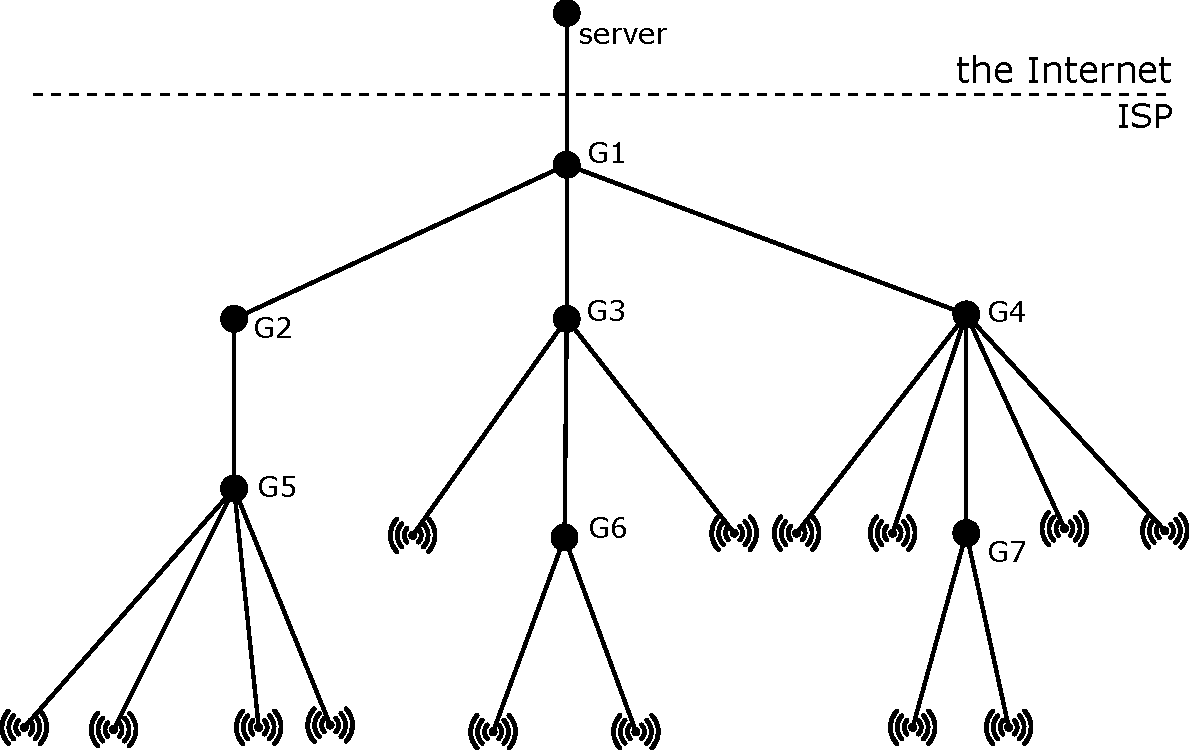
\includegraphics[width=137mm]{drawings/layout}
	\caption{The simulated network topology}
	\label{fig11:sim_layout}
\end{figure}


The simulated network is illustrated in Figure \ref{fig11:sim_layout}. The network is tree-shaped. The topmost node is server, it represents the rest of the Internet. Further, there is part of the infrastructure of an ISP. There are gateway nodes G1-G7. All gateways have 2-5 children. The leafs of this tree are access points (AP) of wireless networks. Finally, 8-12 clients (customers of ISP) are connected to each AP, with the default seed this results in 143 clients. 

Each client is connected to exactly one AP. The clients are connected with 802.11n wifi --- they share the bandwidth. APs and gateways are connected with point-to-point links with 100Mbps bandwidth and 5ms delay. The server is connected to G1 with 200Mbps link with 50ms delay.


The clients download and upload data. All traffic flows between server and one of the clients. There are several types of applications, that model various behaviour real-life clients. The types are listed in table \ref{tab01:traffic}. They vary in transport protocol used, size of single packet and data rate at which they generate traffic. The data rate may be constant --- in that case the application generates packets on regular basis (e.g. it sends a packet every 5 milliseconds). If the application has variable bit rate, it turns itself on and off on irregular basis. The on times and off times are generated randomly.

\begin{table}
	\caption{Types of applications}
	\label{tab01:traffic}
	\centering
	
	
	\begin{tabular}{@{}lllllll@{}}
		\toprule
		Name     & Protocol & Data rate & C/VBR   & directions & Packet         & Priority \\ 
		&          &           &         &            & size(B)        & \\ \midrule
		SSH      & TCP      & 1 kbps    & CBR     & both       & 20             & 1        \\
		VoIP     & TCP      & 60 kbps   & CBR     & both       & 208            & 2        \\
		Game     & TCP      & 100 kbps  & CBR     & both       & 512            & 1        \\
		Stream   & TCP      & 3 Mbps    & CBR     & one        & 1450           & 2        \\
		HTTP     & TCP      & unlimited & VBR     & one        & 256            & 1        \\
		Download & TCP      & unlimited & CBR     & one        & 1450           & 0        \\
		HDIPTV   & UDP      & 10 Mbps   & CBR     & one        & 1450           & 1        \\ \bottomrule
	\end{tabular}
\end{table}


To evaluate MSFC, we ran multiple simulations. Each time, we installed the evaluated scheduler to all nodes (NetDevices) of the simulation. We tested PfifoFast, CoDel, FQ CoDel and MSFC. We have used all schedulers with default parameters, we set the size to bandwidth-delay product. 



\begin{table}[]
	\centering
	\caption{My caption}
	\label{my-label}
	\begin{tabular}{lllll}
		& PfifoFast & CoDel & FQ CoDel & MSFC \\
		Goodput                 &           &       &          &      \\
		Delay                   &           &       &          &      \\
		Jitter                  &           &       &          &      \\
		Differentiated services &           &       &          &     
	\end{tabular}
\end{table}







\section{Discussion}